\documentclass[french, a4paper, 12pt, openany]{report}
% General packages
\usepackage{amsfonts, amssymb, amsthm}
\usepackage{array}
\usepackage{enumitem}
\usepackage{mathtools}
\usepackage{stmaryrd}
\usepackage{empheq, environ} % packages for system environment
\usepackage{calrsfs} % better mathcal letters
\usepackage{graphicx}


% Layout
\usepackage{fancyhdr, fancyvrb}
\usepackage{lastpage}
\usepackage[left=2.0cm, right=2.0cm, top = 2.0cm, bottom = 2.0cm]{geometry}
\usepackage{lettrine, yfonts}
\usepackage{multicol}
\usepackage{minitoc}
\usepackage{hyperref}
\hypersetup{hyperindex=true, colorlinks, linkcolor=blue, urlcolor=blue, citecolor=blue, breaklinks=true}
\everymath{\displaystyle}


% Language
\usepackage[utf8]{inputenc}
\usepackage[T1]{fontenc}
\usepackage{babel}


% Minted
\newcommand{\python}{\mintinline[breaklines=true, breakanywhere=true]{python}}
\newminted{python}{
	linenos=true,
	tabsize=4,
	breaklines=true,
	fontfamily=courier,
	autogobble,
	style=rainbow_dash,
	xleftmargin=5pt,
	xrightmargin=5pt,
	frame=lines
}


% Pagestyle
\everymath{\displaystyle}
\pagestyle{fancy}
\fancypagestyle{plain}


% Customs commands and environnements
\renewcommand{\leq}{\leqslant}
\renewcommand{\geq}{\geqslant}
\renewcommand{\ker}{\mathrm{Ker\,}}
\renewcommand{\vec}{\overrightarrow}
\newcommand{\im}{\mathrm{Im\,}}
\newcommand{\derivative}[2]{\frac{\mathrm{d} #1}{\mathrm{d}#2}}
\newcommand{\enluminure}[2]{\lettrine[lines=3]{\small \initfamily #1}{#2}}
\newcommand{\nnchapter}[1]{
	\chapter*{#1}
	\addstarredchapter{#1}
	\markboth{\uppercase{#1}}{}		
}

\def\restriction#1#2{\mathchoice
              {\setbox1\hbox{${\displaystyle #1}_{\scriptstyle #2}$}
              \restrictionaux{#1}{#2}}
              {\setbox1\hbox{${\textstyle #1}_{\scriptstyle #2}$}
              \restrictionaux{#1}{#2}}
              {\setbox1\hbox{${\scriptstyle #1}_{\scriptscriptstyle #2}$}
              \restrictionaux{#1}{#2}}
              {\setbox1\hbox{${\scriptscriptstyle #1}_{\scriptscriptstyle #2}$}
              \restrictionaux{#1}{#2}}}
\def\restrictionaux#1#2{{#1\,\smash{\vrule height .8\ht1 depth .85\dp1}}_{\,#2}}

\NewEnviron{system}[1][2]
{
	\begin{empheq}[left=\empheqlbrace]{alignat=#1}
        \BODY
    \end{empheq}
}
\NewEnviron{subsystem}[1][2]
{ 
    \begin{subequations}
    \begin{empheq}[left=\empheqlbrace]{alignat=#1}
    	\BODY
    \end{empheq}
    \end{subequations}
}
   
\newtheorem{theoreme}{Théorème}[section]
\newtheorem{definition}[theoreme]{Définition}
\newtheorem{proposition}[theoreme]{Proposition}
\newtheorem{propriete}[theoreme]{Propriété}
\newtheorem{lemme}[theoreme]{Lemme}
\newtheorem{formule}[theoreme]{Formule}
\newtheorem{remarque}[theoreme]{Remarque}
\newtheorem{exemple}[theoreme]{Exemple}

\usepackage{titling}
\usepackage{graphicx}


\title{\sc Modèle de \textsc{Vicsek}}
\author{Alexis {\sc Peyroutet}, Antoine {\sc Royer}}
\date{Janvier – Juin 2023}

\lhead{}
\rhead{\thetitle}
\lfoot{\theauthor}
\cfoot{\thepage\ $|$ \pageref{LastPage}}
\rfoot{L3 PCAME\\2022 — 2023}

\renewcommand{\headrulewidth}{0.4pt}
\renewcommand{\footrulewidth}{0.4pt}


\begin{document}
\makeatletter
\begin{titlepage}
	\centering
	
	
\includegraphics[width=8cm]{images/ut3.png} \hfill 
\includegraphics[width=8cm]{images/uppa.png} \\
	{\large{\sc Licence 3 de Physique, Chimie, Astrophysique, Météorologie et Énergie}} \\
	\rule{0.5\linewidth}{0.4pt} \\
	{\sc Rapport du projet numérique} \\
	
	%\rule{\linewidth}{0.4pt}
	
	\vfill
	{\huge {\sc \@title}} \\ \vspace{1cm}
	{\Large \@author} \\
	
	\vfill 
	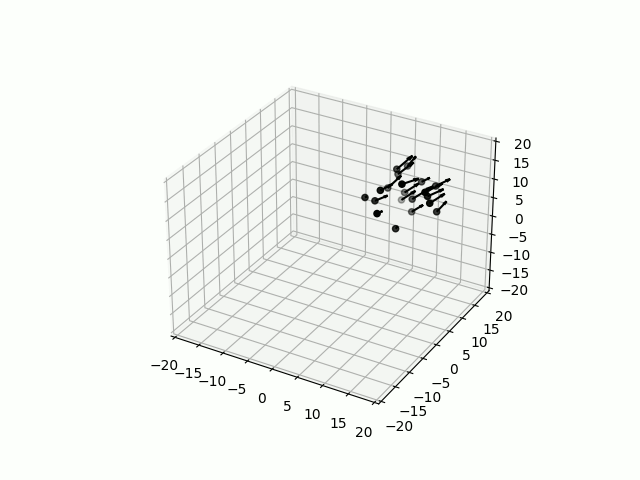
\includegraphics[width=0.7\linewidth]{images/page_garde.png}
	\vfill
	{\Large \@date}
	\rule{\linewidth}{0.4pt}
\end{titlepage}
\makeatother

\tableofcontents

\nnchapter{Introduction}


	Notre sujet est intitulé «~Modèle de \textsc{Vicsek}~». Le but de ce projet numérique est de reproduire de manière numérique le modèle de \textsc{Vicsek}.

	Le modèle de \textsc{Vicsek} a été crée par le scientifique Tamás \textsc{Vicsek}. Il s'agit d'un physicien hongrois connu pour ses contributions à la physique statistique, à la biologie et à la dynamique des systèmes. Il est né le 10 mai 1948 (~74 ans aujourd'hui~) à Budapest. Il est aujourd'hui professeur à l'Université Eötvös \textsc{Loránd} de Budapest. Ce brillant physicien est d'ailleurs un des membres de l'Académie hongroise des sciences et a reçu de nombreux prix pour ses contributions à la physique, notamment le prix \textsc{Széchenyi} (~en 1999~) ou encore le prix Lars \textsc{Onsager} (~en 2020~). \\

	Mais Tamás \textsc{Vicsek} est surtout connu pour son travail sur les systèmes auto-organisés~; ces modèles permettent d'étudier les mouvements collectifs. Il a ainsi travaillé sur le comportement d'agents individuels qui interagissent avec d'autres agents aux alentours, ses observations montrent que des motifs de mouvements collectifs emmergent d'eux-même.
	
	Le groupe se déplace alors de manière coordonnée sans qu'il n'y ait de leader comme on peut l'observer notamment dans la migration des grues. Nous pouvons citer comme exemples~: les bancs de poissons, les regroupements de certains oiseaux, les essaims d'insectes, ou encore le mouvement de foules.

	 Le premier modèle de \textsc{Vicsek} voit ainsi le jour en 1995.\\
	 
	
\chapter{Présentation et explications}	

	Le modèle de \textsc{Vicsek} permet d'étudier un groupe d'agents qui se déplace dans un espace.
	
	Chacun des agents a une vitesse donnée (~en norme et en direction~) et va interagir avec ses voisins. Ce qui concrètement se traduit par des changements concernant la norme et la direction de la vitesse.
	
	Nous nous attendons alors à observer la création d'un mouvement de groupe du aux interactions entre les agents. \\
	
	Cependant, les agents observables dans la vie réelle ne suivent pas toujours le groupe à la perfection, et il peut arriver qu'un agent s'écarte, de manière aléatoire, des autres. C'est pour cela que \textsc{Vicsek} a introduit une notion de bruit dans son modèle. En effet, à chaque pas de temps, chaque agent va prendre la direction moyenne des agents autour de lui et à cette direction va venir se superposer un bruit qui le fera peut-être dévier dans une autre direction.
	
	En augmentant significativement le bruit, le groupe pert son mouvement collectif et les agents prennent alors des directions aléatoires.\\

	Le modèle de \textsc{Vicsek} s'implémente très simplement puisqu'il se réduit à deux équations~: \label{equations} 
	\[ \left\{ \begin{array}{rcl}
		\Theta_{i}(t + \text dt) & = & \Theta_{j |r_{i}-r_{j}|<r} + \eta_{i}(t) \\[0.2cm]
		r_{i}(t + \text dt) & = & r_{i}(t) + v_{i}\Delta t
	\end{array} \right. \]
	dans lesquelles $r_{i}$ la position de chaque individu donnée par un vecteur de position, nous prendrons $i$ comme indice de l'agent en question et $t$ le temps. Nous noterons également $\eta$ le bruit et $\Theta$ pour l’angle définissant la direction de sa vitesse. Ici, $\Theta_{j |r_{i}-r_{j}|<r}$ nous indiquera la direction moyenne des vitesses des agents dans un cercle de rayon $r$. L'indice $j$ repésentera alors l'ensemble des voisins de $i$ compris dans ce cercle.\\

	Ce qui est intéressant, c'est que nous pouvons, en modifiant certains paramètres du système étudié, observer un mouvement de foule plus fort ou plus faible. Nous pourrons alors jouer sur la surface et les dimensions du plan étudié, le nombre d'agent et donc par conséquent la densité de population et même le bruit.\\

	Le modèle de \textsc{Vicsek} est important pour étudier le comportement de certains animaux en biologie ou encore l'étude des foules. Ce modèle peut même être utile à la construction de bâtiment. En effet, le comportement des foules peut être intéressant dans la conception d'entrées et de sorties d'un espace fermé, notamment dans un moment de panique. La foule va s'éloigner du danger est emprunter les sorties. Il est alors crucial de prévoir le comportement des agents pour placer les sorties de manière à ce que le débit d'agent sortant soit le plus important possible.\\
	
	Nous pouvons également retrouver le modèle de \textsc{Vicsek} dans la robotique. C'est un précieux outil pour la technologie du monde moderne. Il peut être utiliser dans des programmes informatiques qui gèrent le déplacement de systèmes de robots (~comme les drones~).\\ 

	C'est avec tout cela que nous essayerons, à travers ce projet, de reproduire numériquement des mouvements collectifs et ainsi étudier le modèle de \textsc{Vicsek}.
	
\chapter{Méthode employée}
\section{Classes et méthodes}

    Pour ce projet, la programmation orientée objet s'est naturellement imposée. Nous utilisons ainsi deux classes appelées \verb|Agent| et \verb|Group| qui fixent respectivement les paramètres de l'agent et du groupe. Assez simplement, la classe \verb|Group| contient une liste d'instances de la classe \verb|Agent| et permet de les représenter dans l'espace et le temps. La classe \verb|Agent| permet d'encapsuler toutes les données de chaque agent~: position, vitesse et direction, bruit, champ de vision etc.
    
	Ainsi, nous pouvons retrouver dans chaque classe, plusieurs méthodes qui vont nous aider à mieux définir les groupes et les agents ainsi qu'à les faire évoluer. \\
  
\section{Création et manipulations d'agents}
	Pour représenter nos agents, nous avons créé une classe qui contient la position de l'agent, sa direction, ainsi que sa vitesse.
	
	À ces paramètres de bases, nous avons rajouté la distance de vision qui permet à chaque agent d'avoir une vue limitée d'une part, mais aussi variable d'un agent à l'autre, ce qui nous permet de simuler une population avec des aveugles par exemple ou des individus d'âges différents (~ce qui n'est pas le cas dans le modèle de \textsc{Vicsek}~) . Les agents ont également un champs de vision unique. Cela caractérise son angle de vue.  
	
	Le bruit d'un agent caractérise l'écart angulaire aléatoire entre sa direction et la direction moyenne de ses voisins. Un bruit fort entraîne donc des écarts importants et les groupes se dissocient plus facilement.
	
	Avec l'apparition des agents répulsifs (voir chapitre~\ref{chap:resultats}), nous avons également rajouté une sensibilité à ces agents, ce qui rend compte d'une peur des agents répulsif. Ainsi un agent normal avec une peur nulle ne fuira pas les agents répulsifs. Nous avons ainsi étudié des groupes avec des valeurs limites de bruits et de sensiblité.
	
	Les agents sont également muni d'un attribut qui caractérise leur type, cela permet de savoir si l'agent est un agent normal, leader, répulsif ou un obstacle. En effet, les obstacles sont gérés comme des agents répulsifs immobiles et qui ne peuvent pas tuer (contrairement aux agents répulsifs). La répulsion stérique n'ayant pas été prise en compte, les agents peuvent théoriquement traverser un obstacle, nous avons dit forcer les obstacles à avoir la priorité sur les autres agents. Autrement dit, si un agent normal fuit un agent répulsif et qu'il voit un mur, il fera demi tour car le mur est plus puissant que l'agent répulsif. Dans ce genre de cas, il arrive que l'agent normal fasse des aller-retours entre le mur et le prédateur jusqu'à sa mort. \\
	
	Les agents sont également munis de plusieurs méthodes qui permettent de les manipuler le plus simplement possible.
	
	Nous avons commencé par définir la soustraction comme étant la distance entre les deux agents, ainsi \verb|agent_1 - agent_2| nous renvoie la distance séparant les deux agents ce qui simplifie les écritures dans la suite du programme.
	
	De manière assez standard nous avons créé une méthode \verb|Agent.copy| qui renvoie une copie profonde de l'objet ce qui nous permet de nous affranchir des problèmes d'alias de Python.
	
	la dernière méthode de cette classe est \verb|Agent.next_step|, elle permet de faire évoluer l'agent en fonction de ses voisins qu'il faut donner en argument. C'est dans cette méthode que sont implémentées les équations en qui régissent le modèle.
	
\section{Création et manipulations de groupes}
	À l'instar des agents, les groupes sont munis d'un certain nombre d'attributs.
	
	Le plus important d'entre eux est sans doute la liste d'agents. En effet, cette liste contient les instances des agents qu'il faut faire évoluer.
	
	Les groupes ont également une liste d'agents morts et qui correspondent aux agents qui ont été touchés par des agents répulsifs. Les stocker permet de faire des statistiques sur ces agents à la fin de la simulation.
	
	Les deux derniers attributs concernent l'espace~: la longueur, la dimension (~2 ou 3~) et la densité du groupe. \\
	
	La classe \verb|Group| contient cependant bien plus de méthodes que les agents.
	
	Tout d'abord, nous avons écrit une méthode qui permet de rajouter des agents au groupe. Cela est pratique en particulier pour rajouter des agents spéciaux. Nous pouvons ainsi générer un groupe de 50 agents et rajouter un agent répulsif.
	
	Comme pour la classe \verb|Agent|, nous avons également créer une méthode de copie profonde qui nous permet de dupliquer le groupe en nous affranchissant des problèmes d'alias.
	
	La méthode \verb|Group.get_neighbours| retrouve tous les agents voisins d'un agent donné en argument en fonction de ses caractéristiques.
	
	Pour la représentation graphique, nous avons deux méthode~: \verb|Group.compute_figure| et \verb|Group.compute_animation| qui renvoient respectivement une image et une animation. Mais, de manière à faire des tests sans forcément avoir une trace sous forme d'image ou d'animation, nous avons également fait une méthode \verb|Group.run| qui permet de faire évoluer le groupe.
	
	La dernière méthode a un sens un peu plus physique puisqu'elle correspond au paramètre d'alignement. Ce dernier est défini pour $N$ agents comme~:
	\[
		\sum_{i=1}^N \frac{\textbf{v}_i}{v_i}
	\]
	où $\textbf v_i$ est le vecteur vitesse de l'agent $i$ et où $v_i$ est la norme ce de même vecteur. Dans son papier \textsc{Vicsek} divise la somme des vitesses par le nombre d'agents multipliés par la norme de la vitesse ce qui présuppose que tous les agents n'ont pas la même vitesse. Dans notre implémentation, nous avons choisit de ne pas imposer une vitesse unique et tous nos agents ont des vitesses qui leur sont propres.	

   
\chapter{Premières interprétations physiques}
\section{Animations en fichier GIF}

   Pour pouvoir observer un mouvement, il est plus utile de regarder une vidéo que des images. Nous avons alors créé une méthode~: \verb|Group.compute_animation| qui utilise la classe \verb|Artist_animation| du module \verb|matplotlib|. Nous arrivions alors à générer des fichiers GIF avec le nombre de frames souhaité.\\
   
   Après avoir généré plusieurs animations avec des groupes de tailles différentes, nous avons pu déjà tirer quelques conclusions. En effet, nous observions des mouvements de groupes. Les agents qui avaient des positions de départ aléatoires, sont influencés les uns les autres selon la distance avec leurs voisins.
   
   On observe d'ailleurs des mouvements collectifs plus importants quand la densité d'agent est plus forte. En revanche, quand les agents sont moins nombreux dans un même espace, nous observons davantage de formations de petits groupes ou des agents solitaires. Nous pouvons régler ce paramètre de densité avec \verb|length| qui correspond à la longueur de l'espace considéré.
   
   Cela s'explique par le fait que les agents ne se voient plus.
	\begin{figure}[!h]
		\centering
		\begin{tabular}{cc}
			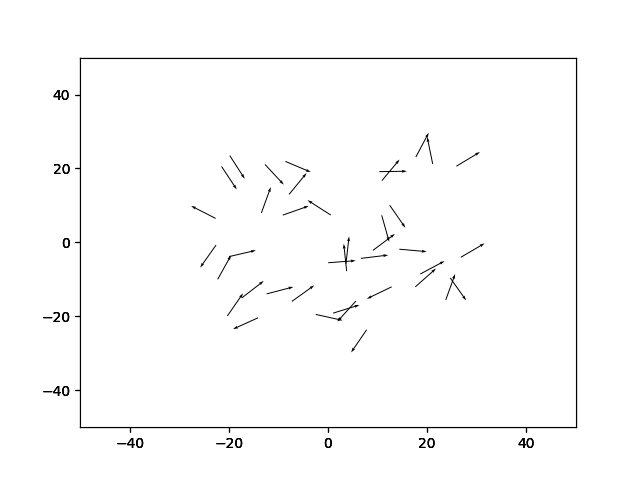
\includegraphics[width=8cm]{images/image_3.png} & 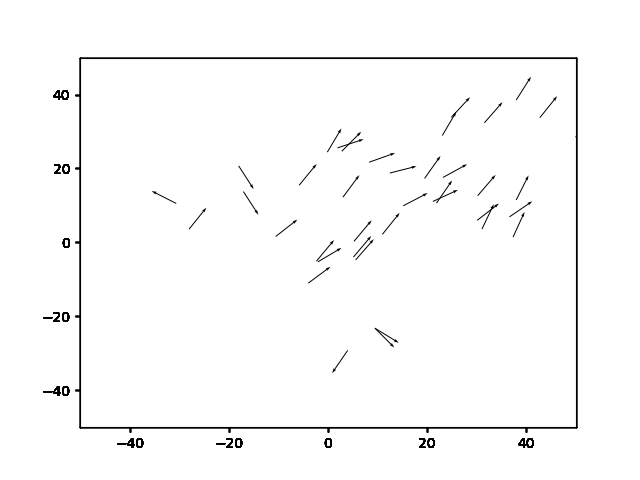
\includegraphics[width=8cm]{images/image_4.png} \\
		\end{tabular}
		\caption{Début et fin d'une animation 2D}
	\end{figure} 

   Nous avons très vite privilégié la représentation 2D pour la suite du projet. En effet, celle-ci permet d'observer plus facilement le comportement des agents, et les différents groupe crées. 
   
   
\section{Mouvements de groupe}

   Pour mieux observer les mouvements de groupe, nous avons décidé de mettre une couleur à nos agents selon leur direction. Cela permet de mieux visuliser les différents groupe et de s'affranchir des flèches qui étaient devenues gênantes pour bien discerner le mouvement collectif à haute densité.\\
   
   Nous avons alors crée une fonction appelée \verb|get_colors|. Avec une boucle \verb|for| et 361 itérations, nous balayons les 360 degrés de l'espace considéré. Avec une suite de \verb|if| et \verb|elif|, nous répartissons la gamme de couleur sur l'ensemble des angles.
   
   Puis, en appelant cette fonction, dans la méthode \verb|get_color| de la classe \verb|Agent|, nous pouvons en fonction de l'angle entre l'horizontale ascendante et le vecteur vitesse de l'agent considéré, associé une couleur particulière.
   
   
   
   Nous avons gardé cette représentation de l'angle des agents pour tout le reste du projet.
   \begin{figure}[!h]
		\centering
		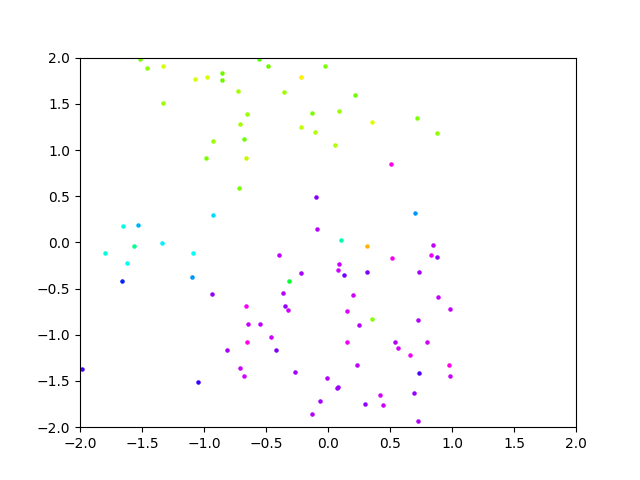
\includegraphics[width=10cm]{images/image_6.png}
		\caption{Image colorée pour la visualisation de groupe}
		\label{couleurs_image}
	\end{figure}  
   
   Sur cette nouvelle figure \ref{couleurs_image}, nous voyons bien les différents groupes crées. On distingue encore mieux les mouvements lors de l'animation.\\
   
   Nous avons d'ailleurs pu observer une organisation intéressante des agents sur certaines animations. En effet, les agents se regroupent premièrement en plusieurs petits groupes (~sur l'image de gauche de la figure \ref{mouvement_grp2}, on discerne en effet trois groupe principaux en violet, vert et cyan~). Enfin, les petits groupes s'unissent pour former un seul et même grand groupe.
   
    \begin{figure}[!h]
		\centering
		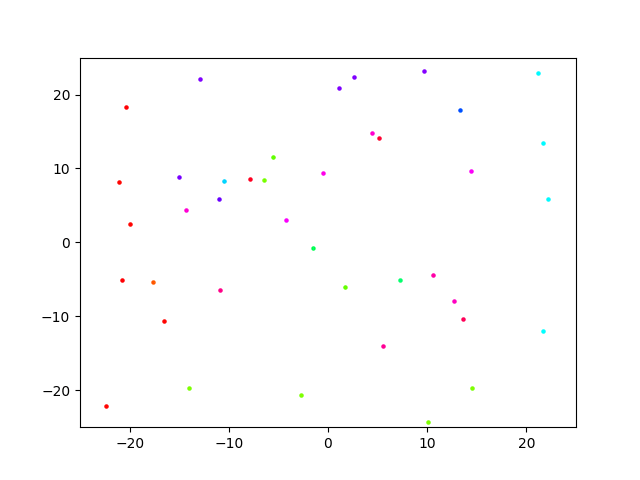
\includegraphics[width=10cm]{images/image_8.png}
		\caption{Image de départ }
		\label{mouvement_grp}
	\end{figure} 
	
   \begin{figure}[!h]
		\centering
		\begin{tabular}{cc}
			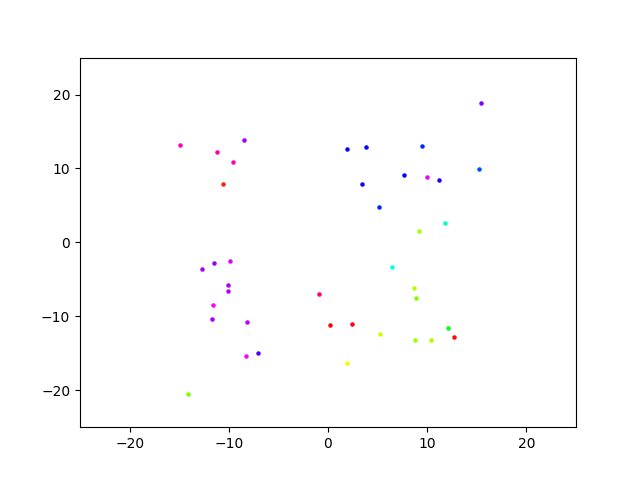
\includegraphics[width=8cm]{images/image_7.png} & 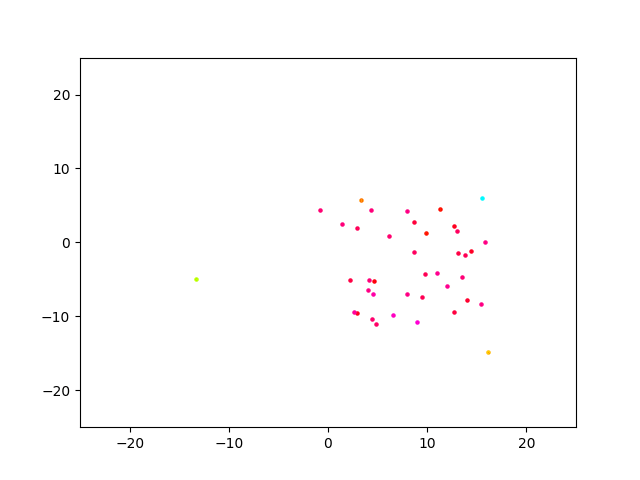
\includegraphics[width=8cm]{images/image_9.png} \\
		\end{tabular}
		\caption{Formations de petits groupe puis d'un seul et même groupe}
		\label{mouvement_grp2}
	\end{figure} 
	
	Ceci montre encore un fois très bien l'influence entre les agents.
\newpage
\section{Paramètres en jeu}
	\subsection{Cône de vision}
	
		Afin de mieux visualiser ce que peut voir un agent en particulier, nous avons alors décidé de rajouter un cône de vision.
     
      Pour ce faire, nous avons utilisé le module \verb|import matplotlib.patches| qui nous a permis de tracer ces cônes en 2 dimensions. Nous nous sommes servis de ce module, qui demande la position et l'angle de vue de l'agent en radian. Nous avons alors converti au préalable l'angle de vue (~paramètre \verb|field_sight|~) en radians.
      
      Puis, avec le module \verb|matplotlib.collections|, nous avons fait apparaître le cône directement sur la figure générée.
		
		Nous sommes ainsi capable de mieux voir comment un agent réagit selon ce qu'il voit. \\
		
		Ainsi, un agent un considéré comme voisin s'il est dans le cône de vision de l'agent testé. En refaisant le même test que précédemment, nous observons que les agents restent alignés moins longtemps.
		
		En effet, les agents étant plus sensible à l'orientation pour voir les autres, si le bruit augmente, les agents vont avoir des déviations angulaires plus importante et peuvent donc perdre de vue les autres agents plus facilement ce qui fait chuter le paramètre d'alignement plus rapidement.
	
   \begin{figure}[!h]
		\centering
		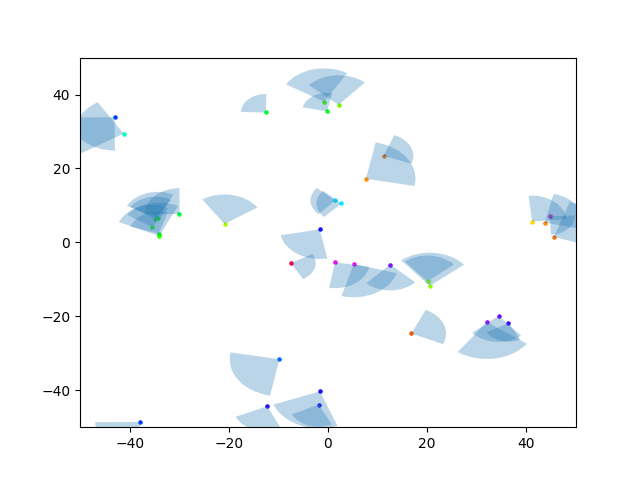
\includegraphics[width=9cm]{images/image_12.png}
		\caption{Image de l'animation générée avec cône de vision}
		\label{cone_vision}
	\end{figure}  
	
	Nous avons cependant préféré retirer la représentation visuelle de ce cône dans la suite du projet. En effet, l'animation générée devenait trop chargée et riche en informations. Il était alors difficile de bien observer le comportement des agents.\\  
  
  \subsection{Paramètre de bruit}
    
   Le bruit correspond à l'influence des voisins sur un agent du groupe. C'est un paramètre essentiel du modèle de \textsc{Vicsek}. Nous le retrouvons (~sous la lettre grecque $\eta$~)  dans les équations qui définissent le modèle dont nous avons parlé dans le chapitre \ref{equations}.\\
   
   Plus le bruit est fort, plus celui-ci aura tendance à ne pas s'occuper de ses voisins et prendre sa propre direction. A l'inverse, avec un bruit qui tend vers zéro, l'agent aura tendance à imiter ses voisins et prendre une direction similaire aux agents autour de lui. \\
    
   Nous avons déjà pu observer l'impact du bruit sur les populations. Nous voyons alors que ce paramètre est capital pour l'observation de mouvements collectifs. Si celui-ci est trop fort, les agents feront route seuls et ne s'occuperont pas du mouvement des voisins. En revanche, les mouvements collectifs seront davantages présents avec un bruit qui tend vers zéro.
\newpage
Par exemple, en regardant cette figure~:


   \begin{figure}[!h]
		\centering
		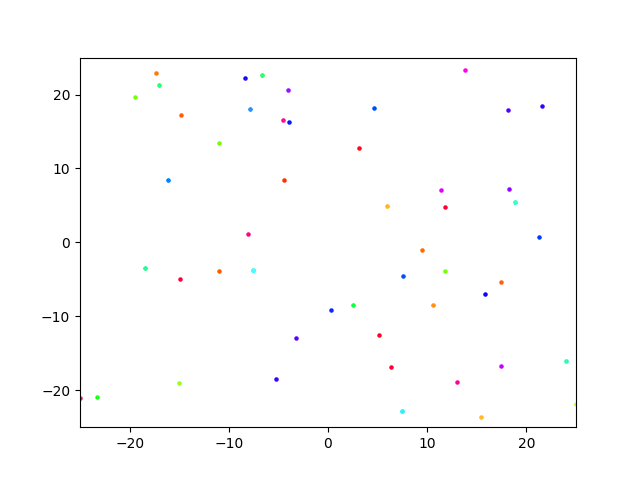
\includegraphics[width=8cm]{images/image_10.png}
		\caption{Visualisation de l'impact du bruit (~bruit fort dans ce cas~)}
		\label{bruit}
	\end{figure}  

	
Nous voyons bien ici que les agents ont des directions plutôt différentes. Nous avons un bruit qui est fort dans ce cas, et nous remarquons que les agents ont tendance à prendre des directions sans s'occuper de leurs voisins. Il est alors évident que le bruit est un paramètre essentiel dans le modèle de \textsc{Vicsek}.
   
\chapter{Résultats expérimentaux} \label{chap:resultats}
\section{Résultats historiques de \textsc{Vicsek}}
\subsection{Paramètre d'alignement en fonction du bruit} 
	Nous avons commencé par chercher à reproduire les résultats obtenus par \textsc{Vicsek} en reprenant les mêmes paramètres.
	
	Chaque agent n'est ainsi influencé que par ses plus proches voisins et évolue dans un espace torique. En laissant la densité constante et en faisant varier le bruit pour voir son influence sur le paramètre d'alignement, nous observons alors un profil de transition de phase.
	
	Sur la figure suivante chaque points est la moyenne sur cinq mesures de 200 pas et 50 agents.
	\begin{figure}[!h]
		\centering
		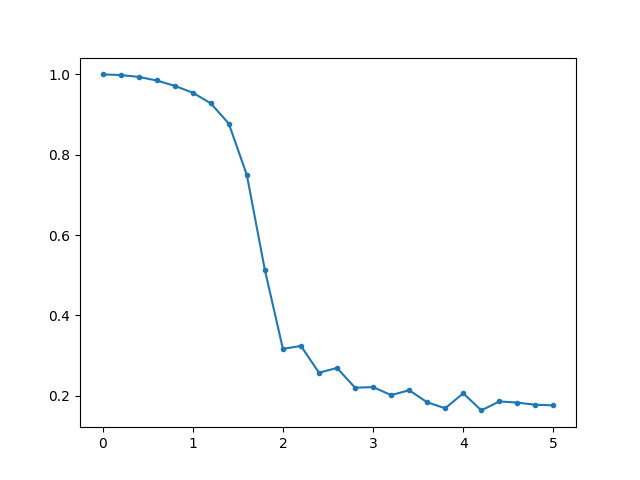
\includegraphics[width=12cm]{images/bruit_4.png}
		\caption{Paramètre d'alignement en fonction du bruit}
	\end{figure}
	
	\textcolor{red}{\textbf{Mettre aussi une figure avec différents nombre d'agent et LEGENDER LES AXES QUI N'EN ONT PAS}}
	Pour un bruit très faible, les agents sont alignés avec un paramètre d'alignement de 1 ce qui est cohérent puisqu'ils vont s'aligner sans aucune part d'aléatoire. Pour un bruit élevé, ce qui correspond en fait à une probabilité d'avoir une déviation angulaire importante par rapport à la direction moyenne, les agents sont très peu alignés pour un même nombre d'itération. \\
	
	Nous avons ici exactement les mêmes résultats que ceux obtenus par \textsc{Vicsek} et son équipe.\\
	
	Nous en avons d'ailleurs profité pour mesurer l'effet du cône de vision sur le paramètre d'alignement, nous avons tracé ce graphe avec 50 mesures par points sur la figure \ref{cone_vision_alignement}. 
	
	Nous pouvons ainsi constater que le cône de vision précipite la transition de phase entre un état parfaitement ordonné et un état chaotique. Cela est logique puisqu'avec l'augmentation du bruit, les agents peuvent prendre des trajectoires de plus en plus aléatoires. Ses voisins peuvent alors sortir du cône de vision, ce qui change radicalement la manière dont l'agent se déplace.
	
	 \begin{figure}[!h]
		\centering
		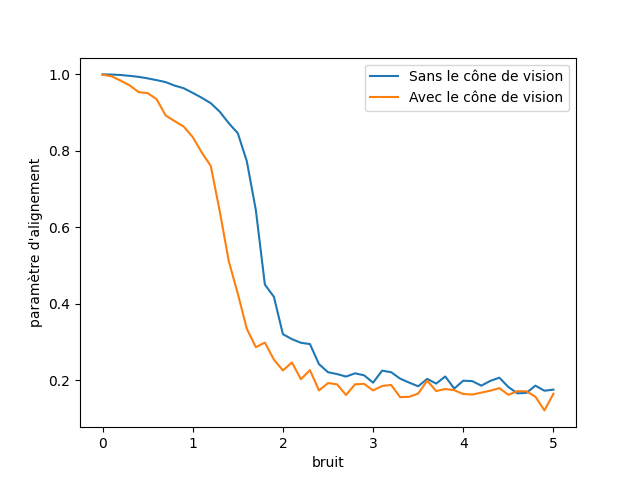
\includegraphics[width=10cm]{images/bruit_comparaison[50 mesures par pts].png}
		\caption{Effet du cône de vision sur le paramètre d'alignement}
		\label{cone_vision_alignement}
	\end{figure}
    
    \subsection{Paramètre d'alignement en fonction de la densité}

    \textsc{Vicsek} avait aussi mesuré le paramètre d'alignement en fonction de la densité d'agent dans l'espace (~avec un bruit constant~). En traçant le paramètre d'alignement en fonction de la densité, nous obtenons pas excatement la même figure que \textsc{Vicsek} même si cela s'en rapproche.
      
       \begin{figure}[!h]
		\centering
		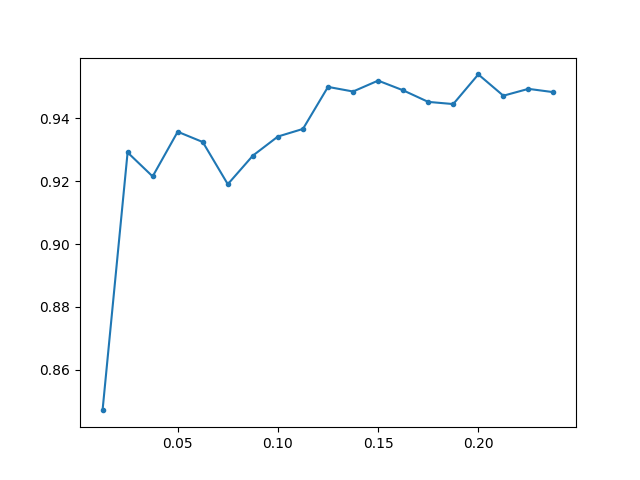
\includegraphics[width=10cm]{images/densite_1[noise=1].png}
		\caption{Paramètre d'alignement en fonction de la densité d'agent (~bruit=1~)}
		\label{densité_alignement}
	\end{figure}
	
	Nous pouvons tout de même en déduire que plus le nombre d'agent est élévé dans un même espace (~et donc la densité aussi~), plus les agents s'aligneront sur la même direction rapidement. Nous pouvons même rajouter qu'à partir d'une valeur de densité d'environ de 0.13 agents par unité d'espace. 
	
	Nous n'avons pas clairement identifié quel paramètre différait entre notre modèle et celui de \textsc{Vicsek}. Cependant, il est probable qu'ils s'agisse d'une différence dans la manière de faire évoluer le groupe. En effet, pour chaque point nous repartons de zéro en regénérant un nouveau groupe alors qu'il est possible que \textsc{Viscek} garde le même groupe en rajoutant des agents pour faire augmenter la densité.
    \newpage
    \section{Au-delà du modèle de \textsc{Vicsek}}
    \subsection{Création d'un agent leader}
       Nous avons maintenant voulu nous écarter un peu du modèle de \textsc{Vicsek}, en étudiant un nouveau type de mouvement collectif. Nous avons alors crée un nouveau type d'agent, dit leader, qui influence davantage les agents normaux. Nous pouvons définir à quel point celui-ci à de l'influence (~nous pouvons choisi une influence équivalente à n agents~).\\
       
       Nous avons alors crée le paramètre \verb|agent_type| pour différencier les agents. Ainsi, il nous faut préciser l'indice correspondant à l'agent que l'on veut créer avec \verb|agent_generator|. Il nous faudra ensuite rajouté cette agent au groupe créer avec la méthode \verb|add_agent|. Nous avons décidé que agents classiques sont de type 0 et les agents leader de type 1.\\
       
       Avec l'apparition de ce nouveau type d'agent, nous nous attendions à observer des groupe en forme de pyramide. C'est-à-dire une organisation hiérarchique des agents pour créer un mouvement de groupe. Nous pouvons par exemple observer ce comportement chez certains animaux, notamment lors de la migrations des grues. 
       
   Nous avons choisi de représenter l'agent leader en noir.
   \begin{figure}[!h]
		\centering
		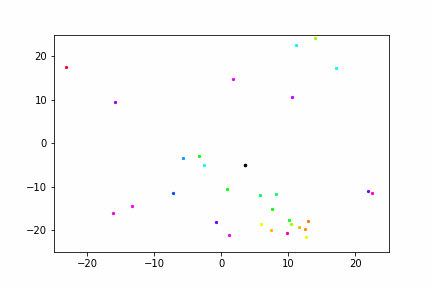
\includegraphics[width=10cm]{images/image_15.png}
		\caption{Effet observée avec un agent leader}
		\label{leader}
	\end{figure}  
	
	   En effet, nous avons observé plusieurs fois une organisation en «~triangle ou en arc de cercle~», comme une sorte de hiérarchie. L'agent leader produit un mouvement de groupe organisé différemment de ce qu'on a pu observer dans le modèle de \textsc{Vicsek}.
	   
	   Ainsi, cela montre que le mouvement collectif peut être amené de différentes manières et qu'il n'y a pas de méthode unique pour un déplacement d'un ensemble d'agent.\\
    
  
       Nous avons d'ailleurs pu observer quelque chose d'intéressant. En effet, sur une animation, nous pouvons voir un groupe d'agent qui suit l'agent leader pendant un moment. Mais, ce groupe croise un autre groupe d'agent. Les agents qui suivait l'agent leader se sont mis subitement à suivre le nouveau groupe. 
       
       \begin{figure}[!h]
		\centering
		\begin{tabular}{cc}
			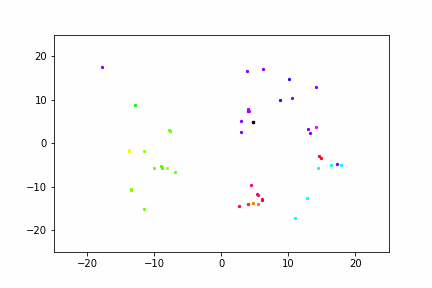
\includegraphics[width=8cm]{images/image_13.png} & 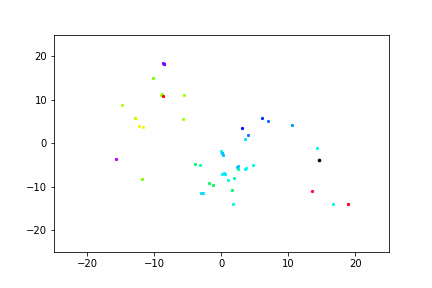
\includegraphics[width=8cm]{images/image_14.png} \\
		\end{tabular}
		\caption{Situation intéressante avec un agent leader}
	\end{figure}
       
       Ainsi, nous en déduisons que le groupe a eu plus d'influence que l'agent leader à ce moment là.
       
       
   \subsection{Mise en place d'une prédation et du paramètre de sensibilité}
       
       Nous avons trouvé intéressant de rajouter des agents dit répulsifs, qui joue le rôle de prédateurs. Ces nouveaux agents sont plus rapides que leurs proies. Ainsi, nous avons pu voir comment s'organisent les agents face à la menace.
       
       Nous avons choisit de paramétrer la réaction des agents quand cet agent répulsif rentre dans leur cône de vision. L'agent prendra immédiatement le vecteur de sens opposé à celui vers l'agent répulsif. Nous avons choisit de représenter les agents répulsifs en noir.\\
       
       Pour créer ce type d'agent, il nous faut préciser \verb|agent_type = 2| dans la méthode \verb|agent_generator|.\\
       
       Avec cette expérience, nous constatons que le mouvement de groupe est toujours présents avec un seul agent répulsif. Cet effet collectif est même souvent renforcé. Les agents fuient dans la même direction, tout en se servant de leur influence les uns sur les autres.
       
        Cependant, lorsqu'il y a plusieurs agents répulsifs, le mouvement collectif n'est plus observé ou très peu. Ces prédateurs (~qui prennent des directions différentes~)  sèment la panique au sein du groupe qui pert visiblement toute cohésion. Chaque agent développe alors un instinct de survie qui le pousse à fuir. La panique et la fuite prennent visiblement le pas sur la cohésion de groupe (~cf. figure \ref{repulsifs_agents}~).\\
       
     \begin{figure}[!h]
		\centering
		\begin{tabular}{cc}
			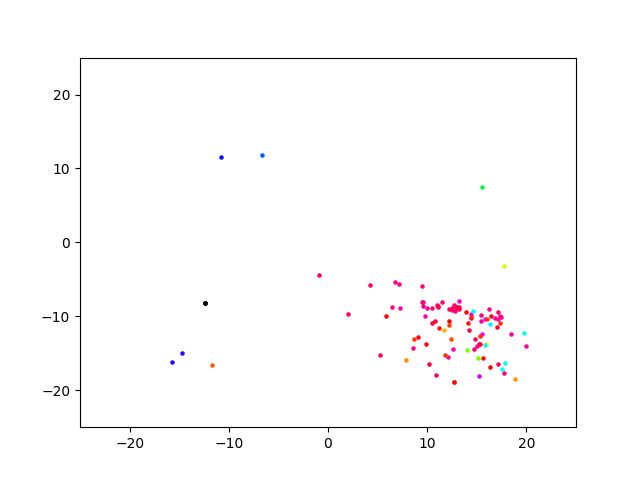
\includegraphics[width=8cm]{images/image_17.png} & 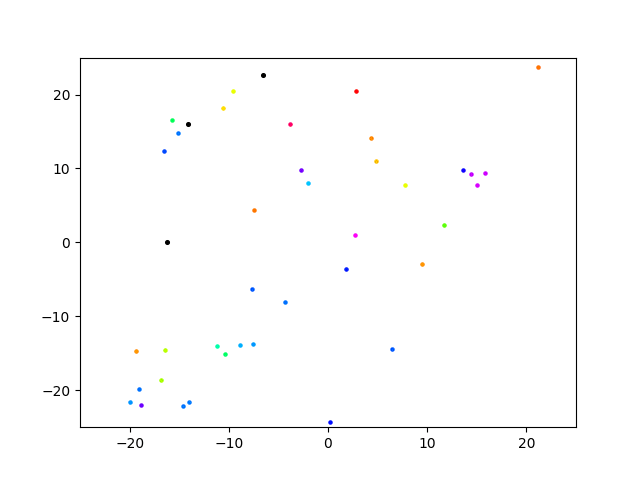
\includegraphics[width=8cm]{images/image_16.png} \\
		\end{tabular}
		\caption{Effet d'un (~à gauche~) ou plusieurs agents répulsifs (~à droite~) sur le groupe}
		\label{repulsifs_agents}
	\end{figure}
       
   Nous avons ensuite décidé de rajouter un nouveau paramètre que nous appelons \verb|fear| dans notre code. Il s'agit de la sensibilité des agents face aux prédateurs, c'est à dire à la peur des agents pour les agents répulsifs. 
   
   Ainsi, les agents prennent plus facilement la fuite face aux prédateurs.      
   

	\subsection{Système évolutif}
	
		En ajoutant des agents répulsifs, nous avons eu l'idée de créer un système de «~mort~» où les agents touchés par un agent répulsifs sont retirés de la liste des agents et placés dans un autre attribut du groupe. Cela permet notamment de comparer les caractéristiques des agents morts avec celles des survivants et de voir quels paramètres permettent de survivre. En mettant des valeurs limites pour le bruit et la sensibilité aux agents répulsifs et en moyennant les résultats sur 10 mesures, nous obtenons les résultats suivants~:\\
		
		\begin{tabular}{|c|c|c|} \hline
		\centering
			bruit & sensibilité & pourcentage de survivants \\ \hline
			1 & 0 & 30 \\ \hline
			0 & 1 & 79 \\ \hline
			1 & 1 & 86 \\ \hline
			0 & 0 & 39 \\ \hline
		\end{tabular}\\

   Nous voyons bien que statistiquement, les agents ont plus de chance de survivre avec un bruit et une sensibilité à 1. En effet, dans ce cas là, les agents avec une grande sensibilité cherche à fuir à tout prix le prédateur. De plus, le bruit fort fait que les agents ne cherche pas à imiter leurs voisins, ce qui ne perturbe pas la fuite qu'il avait entrepris. 
   
   Cependant, en enlevant le bruit, nous voyons tout de même que le pourcentage de survivant reste très élevé. La sensibilité est un élément clé pour la survie des agents.\\

  Au contraire, les agents ont peu de chance de survie avec un bruit fort et un sensibilité nulle. En effet, les agents n'ont pas peur de leurs prédateurs, ce qui devient très dangeureux. De plus, le bruit élevé, fait qu'il n'y a aucun mouvement de groupe.
  
  Cependant, en retirant le bruit, nous voyons le que pourcentage de survivant est à peine plus haut. Nous revenons à la même conclusion~: la sensibilité est un élément clé pour la survie des agents.
  

\subsection{Ajout d'obstacles}

   De plus, nous avons voulu voir comment réagissent les agents face à des obstacles. Nous voulions voir le mouvement de groupe est conservé. 
   
   Cette approche permet de se placer dans des conditions encore plus réalistes. Par exemple, un banc de poissons peut rencontrer des rochers lors de son déplacement. 
   
   Nous avons alors crée des murs, qui font office d'agents répulsifs immobiles. A leur vue, les agents font marche arrière pour éviter l'obstacle. \\
   
   Pour créer ces murs, il nous faut préciser \verb|agent_type = 3| dans la méthode \verb|agent_generator|.\\
   
	\begin{figure}[!h]
		\centering
		\begin{tabular}{cc}
			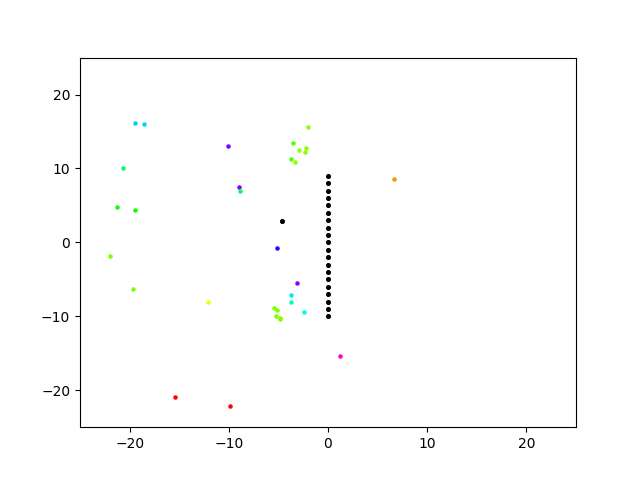
\includegraphics[width=8cm]{images/image_19.png} & 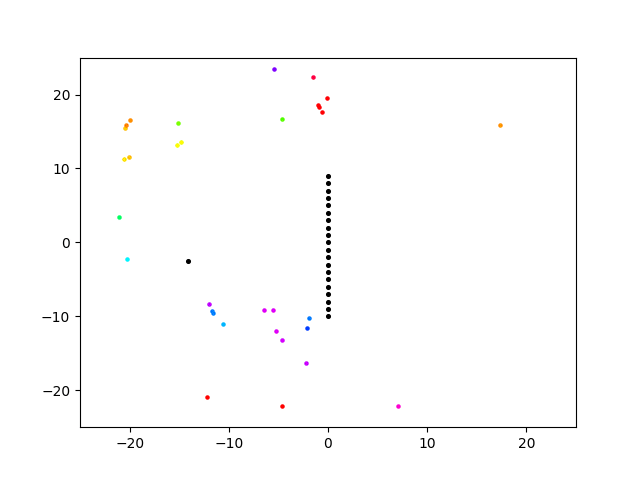
\includegraphics[width=8cm]{images/image_18.png} \\
		\end{tabular}
		\caption{Effet d'un obstacle sur le mouvement des agents (~arrivée des agents vers le mur à gauche, directions prisent par les agents après avoir vu le mur à droire~)}
		\label{obstacles}
	\end{figure}

	Nous voyons bien que les agents rebroussent un peu chemin. En réalité, nous pourrions plutôt nous attendre à ce que le groupe contourne l'obstacle. Il y a tout de même quelques agents qui ont visiblement contourné l'obstacle, mais la majorité du groupe fait demi-tour.
	
	
\nnchapter{Conclusion}


\end{document}
